\documentclass[12pt]{report}
\usepackage{graphicx}
\usepackage{color}


\begin{document}



\chapter{Biochimie}

\includegraphics[width=350]{biochimie_head_fr.jpg} 
\newpage
\section{Introduction}
La biochimie implique l'étude des processus chimiques qui se produisent dans les organismes vivants dans le but ultime de comprendre la nature de la vie en termes moléculaires \cite{ref5} . Les études biochimiques reposent sur la disponibilité de techniques analytiques appropriées et sur l'application de ces techniques à l'avancement des connaissances sur la nature, et les relations entre les molécules biologiques, en particulier les protéines et les acides nucléiques, et la fonction cellulaire \cite{ref5} . Ces dernières années d'importants progrès ont été réalisés dans notre compréhension de la structure et de l'expression des gènes et dans l'application de techniques telles que la spectrométrie de masse à l'étude de la structure et de la fonction des protéines.
Le projet du génome humain en particulier a été à l'origine de développements majeurs dans la compréhension de nombreuses maladies humaines, en particulier le cancer, et dans l'identification de stratégies pouvant être utilisées pour lutter contre ces maladies \cite{ref5} .\\aujourd'hui les grandes recherches scientifiques engagés dans la recherche biochimique et biotechnologie L'objectif principal  est de comprendre comment les biomolécules et leurs interactions génèrent les structures et les processus biologiques observés dans les cellules, pour la compréhension des organismes en général.
\newpage
\section{Biochimie}
\subsection{Définition}
La \textbf{biochimie} est le domaine où se rencontrent chimie et biologie, La biochimie étudie donc particulièrement la corrélation entre la structure des molécules naturelles et les conséquences sur leur activité \cite{ref6} .\\
La biochimie permet de comprendre selon quels "processus chimiques" fonctionnent les organismes vivants, des plus simples comme les bactéries et les virus, jusqu'aux plus complexes, comme les insectes, les mammifères et surtout les humains  \cite{ref6}  .
\subsection{Biologie}
\subsubsection{Définition}
La \textbf{biologie} est la science du vivant. Elle recouvre une partie des sciences de la nature et de l'histoire naturelle des êtres vivants  \cite{ref6} .\\
\begin{figure}[h]
\begin{center}

\includegraphics[width=300]{bio.jpg}
\caption{science du vivant}
\end{center}

\end{figure}


\subsection{La Chimie}
\subsubsection{Définition}
La \textbf{chimie} est une science de la nature qui étudie la matière et ses transformations,  et plus précisément les processus qui changent ou modifient l'identité de ces particules ou molécules de matière, dénommés réaction chimique, transformation, interaction, etc  \cite{ref6} .

\subsection{Les domaines de la biochimie}
la biochimie généralement est utilisé dans nombreuses domaines autour de l'organismes vivants telle que:
\begin{enumerate}
\item \textbf{pharmacologie} 
\item médecine
\item toxicochimie
\item génie génétique
\item structure des molécules
\end{enumerate}
Par exemple, la connaissance des mécanismes d'action d'une molécule sur un organisme permet l'élucidation de sa toxicité. Ce champ de recherche est celui de la toxicochimie  \cite{ref6} .

\section{pharmacologie}


\subsection{Définition}
La \textbf{pharmacologie} est la science de synthèse, emprunte des méthodes à l'ensemble des disciplines biologiques et physico-chimiques. Elle apporte les bases nécessaires à l'étude des mécanismes d'action des médicaments et des mécanismes de régulation des fonctions de l'organisme \cite{ref7}.
\subsection{pharmaceutique}
La biologie est l'un des sciences plus large et plus couteuse aux domaines des recherches scientifiques et parmi ces domaines la recherche pharmaceutique qui basent sur la production des médicaments et de trouvées nouveaux molécules. Le coute de la recherche augment car les molécules les plus faciles à trouvées ont déjà été utilisées, plus d'un milliard d'euros par médicament et le criblage en france. Les laboratoires doivent désormais s'intéresser à des molécules plus grosses, plus complexes \cite{ref7} .

\subsection{L'objectif de pharmaceutique}
les \textbf{médicaments} occupe une place importante dans l’exercice de la médecine \cite{ref7}.\\
La pharmacologie, qui se définit comme la science du médicament, contribue de manière incontournable à la compréhension des effets thérapeutiques attendus ou des effets indésirables observés lors de la prescription du médicament.\\On distingue :
\begin{enumerate}
\item Comprendre les bases pharmacologiques 
\item  la production des médicaments et de trouvées un nouveaux médicament

\end{enumerate}

\subsection{Qu'est ce qu'un médicament}
Il s'agit  de tout produit pouvant être administré à l'homme ou l'animal en vue  diagnostic médical  de restaurer, corriger ou modifier leur fonctions organiques \cite{ref7} . 
\begin{figure}[h]
\begin{center}

\includegraphics[width=300]{med.jpg}
\caption{Médicament}
\end{center}

\end{figure}


\subsection{Le développement du médicament}
 il y a plusieurs étape telle que :
\begin{enumerate}
\item Produire la molécule sélectionnée (principe actif) en quantité satisfaisante.
\item Tester le candidat-médicament, pour évaluer ses effets d'efficacité et ses effets indésirables (études précliniques). 
\item Rendre la molécule administrable sous une forme adaptée (comprimé, solution pour injection, patch, sirop, crème…).
\item Tester (si les étapes précliniques sont satisfaisantes), le médicament chez l'homme, dans le cadre d'essais cliniques \cite{ref7}.
\end{enumerate}
\subsection{Dénomination des médicaments}
On distingue plusieurs noms pour un médicament :
\begin{enumerate}
\item Le nom chimique qui correspond à la formule chimique exemple : acide acetyl salicylique
\item la dénomination commune international :aspirine
\item Les noms commerciaux :Aspegic ,Kardegic ,etc.
\end{enumerate}
\newpage
\section{Les molécules}
\subsection{Définition}
\textbf{Une molécule} est une structure de base de la matière. L'Union internationale de chimie pure et appliquée définit la molécule comme une entité électriquement neutre comprenant plus d'un atome,  C'est l'assemblage chimique électriquement neutre d'au moins deux atomes, différents ou non, qui peut exister à l'état libre \cite{ref8} .\\
\begin{figure}[h]
\begin{center}
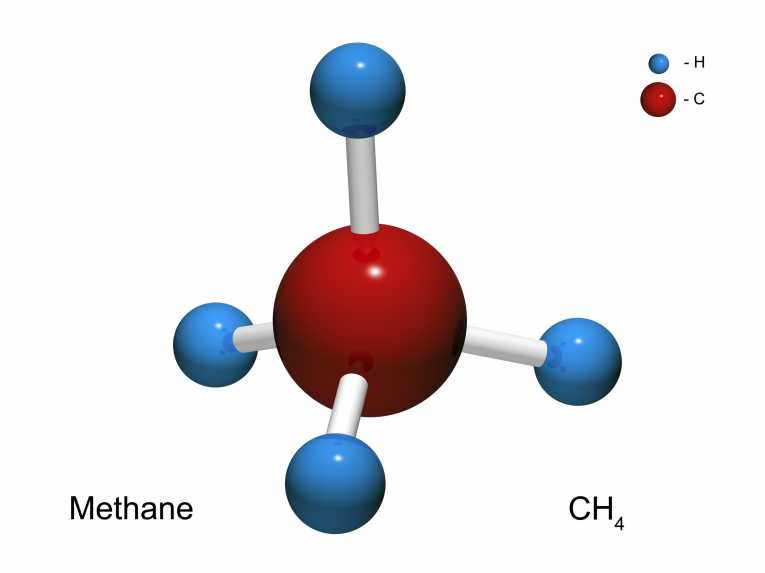
\includegraphics[width=300]{mol.jpg}
\caption{Molécule de methane}
\end{center}
\end{figure}

\subsection{Types particuliers de molécules}
\begin{enumerate}
\item L'étude des composés biochimiques a conduit les chimistes à distinguer les molécules organiques et inorganiques. 

\item Une molécule élémentaire ou \textbf{homonucléaire } est une molécule constituée d'un seul type d'atomes, par exemple le dioxygène (O2). 

\item Une molécule polaire ou \textbf{apolaire} est respectivement une molécule ayant un moment dipolaire résultant non nul (cas de la molécule d'eau) ou nul.

\item Molécule médicamenteuse : on appelle abusivement molécule la substance active d'un médicament (par opposition à son nom de marque).

\item Une molécule \textbf{amphiphile} est une molécule ayant une ou plusieurs parties hydrophiles et une ou plusieurs parties hydrophobes.

\end{enumerate}

\subsection{Le niveau moléculaire}
La structure des organismes biologiques qui constituent la biosphère peut être décomposée en plusieurs niveaux d'organisation : atomique, moléculaire, cellulaire, tissulaire, organique, des systèmes nerveux, et enfin celui de l'organisme dans sa totalité fonctionnelle. L'étude du niveau des molécules permet de comprendre le fonctionnement de la cellule, qui est l'unité fonctionnelle élémentaire du vivant \cite{ref8} .

\subsection{Molécule dans le milieu médicament}
On utilise souvent le terme de molécule pour parler du principe actif d'un médicament, Il ne faut pas confondre l'idée ancienne de principe actif, associée à celle de sa purification réalisée à partir de substances naturelles, avec celle moderne de molécule. S'il existe encore des médicaments qui contiennent des principes actifs extraits de plantes, notamment la plupart des produits pharmaceutiques modernes contiennent des substances actives dont on connaît bien la structure chimique de leur molécule \cite{ref8}. 
\newpage
\section{QSAR}
\subsection{introduction}
Le point de départ consiste à identifier une méthode efficace pour trouver un candidat-médicament actif sur une cible biologique. plus lorsque les propriétés ou structures physiochimiques sont exprimées par des chiffres, on peut proposer une relation mathématique, ou relation quantitative structure à activité, entre les deux. L'expression mathématique obtenue peut alors être utilisée comme moyen prédictif de la réponse biologique pour des structures similaires \cite{ref9} .

\subsection{Définition}
les molécules similaires ont une activité similaire. Le principe des méthodes \textbf{Qsar} consiste à mettre en place une relation mathématique à l'aide de méthodes d'analyse des données, relient des propriétés moléculaires microscopiques appelées descripteurs, à un effet expérimental (activité biologique, toxicité), pour une série des composé chimiques similaires \cite{ref9}.\\
Qsar la plus commune est de la forme : activité = f(propriétés physico-chimiques et/ou structurales).\\
\begin{figure}[h]
\begin{center}

\includegraphics[width=300]{qsar22.png}
\caption{Stilbene}
\end{center}
\end{figure}

\subsection{Domaine d'application}
L'utilisation de modèles \textbf{QSAR} pour la gestion du risque chimique s'accroissant régulièrement et étant aussi utilisé pour des visées réglementaires (en Union européenne : enregistrement, évaluation et autorisation des produits chimiques), il est crucial d'être capable d'affirmer la pertinence des prédictions. L'espace des descripteurs chimiques engendré par un ensemble spécifique de produits chimiques est appelé domaine d'applicabilité, qui permet d'indiquer lorsqu'un composé peut être prédit \cite{ref9}.

\subsection{Descripteur}
\textbf{Les descripteurs} basés sur la composition chimique de la molécule, les topologiques, obtenus à partir de la structure bi-dimensionnelle (table de connectivité des atomes de la molécule).
\\
\begin{figure}[h]
\begin{center}
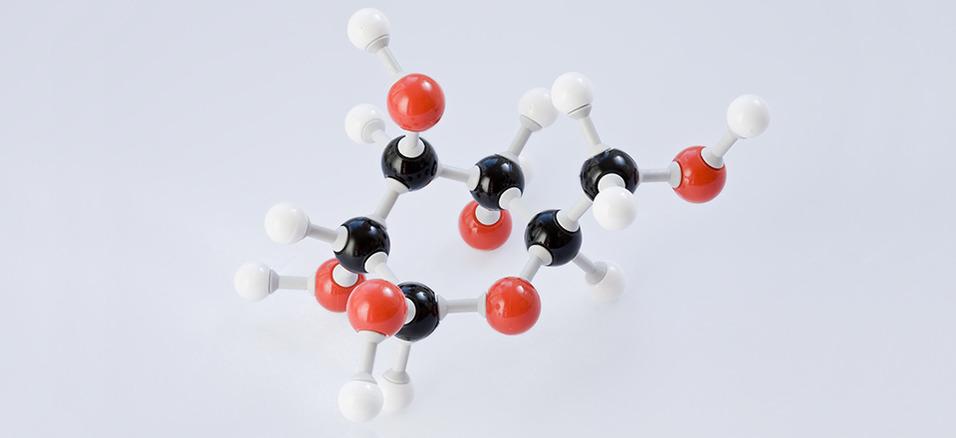
\includegraphics[width=300]{des.jpg}
\caption{Descripteur chimique}
\end{center}
\end{figure}
\subsection{Composition chimique}
La matière étant constituée en général de plusieurs corps purs (composés chimiques et corps simples), la composition chimique d'un produit fournit la quantité ou la proportion de chacun des corps purs qui le composent ; on les appelle de manière générique des composants \cite{ref9}.

\subsection{Activité biologique}
\textbf{l'activité} biologique est l'ensemble de toute les propriété moléculaire, propriété physique. l'activité biologique peut être exprimée de manière quantitative, comme pour la concentration de substance nécessaire pour obtenir une certaine réponse biologique \cite{ref9} .
\subsection{RSA et paradoxe RSA }
Le postulat de base pour les hypothèses sur des objets chimiques est que des objets similaires ont des activités similaires. Ce principe est appelé relation structure-activité (RSA, ou SAR pour structure-activity relationship en anglais). Le problème sous-jacent est donc la définition d'une petite différence sur un niveau moléculaire, chaque type d'activité, comme la réaction chimique, la biotransformation, la solubilité, l'activité de cible et d'autres encore, peuvent dépendre d'une autre différence.En général, l'intérêt est plus de trouver de fortes tendances. Les hypothèses avancées reposent habituellement sur un nombre fini de données chimiques. Ainsi, le principe d'induction devrait être respecté afin d'éviter les hypothèses surapprises et les interprétations erronées et inutiles sur les données chimiques/structurales \cite{ref9}.\\
Le paradoxe SAR est le fait que toutes les molécules similaires ne montrent pas des activités similaires. 

\subsection{Qsar en chimie}
Une des premières applications de la Qsar concernait la prédiction des points d'ébullition.Il est bien connu par exemple que pour une famille de composés chimiques, particulièrement en chimie organique, il existe une corrélation forte entre la structure et les propriétés observées \cite{ref9}.

\subsection{Qsar en biologie}
L'activité biologique des molécules est mesurée habituellement au moyen d'essais afin d'établir le niveau d'inhibition d'une transduction de signal ou d'une voie métabolique particulière. Les produits chimiques peuvent être biologiquement actifs par leur toxicité. La recherche de médicament implique parfois l'utilisation de la Qsar afin d'identifier les structures chimiques pouvant présenter de bons effets inhibiteurs sur des cibles spécifiques et possèdent une faible toxicité.

\section{Conclusion}
Tout a long de ce chapitre, nous avons pu nous rendre compte de l'avancée impressionnante de la science moderne dans le domaine de la biochimie. L'évolution de la biochimie a une influence non négligeable sur la société humaine. Elle pourrait la transformer radicalement, pour le meilleur ou pour le pire. Face aux nombreux bénéfices qui en résulteraient, les valeurs morales nous empêchent d'aller trop vite.
L'intelligence artificielle (IA) a transformé durablement l'industrie des sciences biologiques, de la médecine et de la santé. Deep Learning accélérées par les GPU peuvent être utilisées pour concevoir des réseaux de neurones encore plus sophistiqués afin d'optimiser les applications de biochimie et de recherche pharmaceutique dans de nombreux domaines .
Dans le prochain chapitre, nous allons présenter quelque concepts et définitions sur  le deep learning et les différentes utilisations dans la vie biochimie.


\end{document}
